% !TEX program = XeLaTeX
%%=======================================================================
%% HUAS-Beamer-Blue-EN.tex —— 湖南文理学院 Beamer 模板英文演示（冷色调·蓝白，English demo）
%%=======================================================================
%% Compile: latexmk -xelatex HUAS-Beamer-Blue-EN.tex (bibtex handled automatically)
%%   or xelatex HUAS-Beamer-Blue-EN.tex (with references: xelatex -> bibtex -> xelatex x2)
%%
%% ★ How this demo is organised ★
%%   Neutral academic-report / template-demo narrative: every slide presents
%%   one category of layout elements (lists / columns / figures / blocks /
%%   theorems / formulas / tables / code / citations / hyperlinks ...), with
%%   sample material adapted from common template examples (research contents
%%   and progress, completed work, future work, problems and solutions).
%%   Replace the sample text page by page with your own.
%%   Same content as HUAS-Beamer-EN.tex; only the theme loading line differs ([blue]).
%%
%% ★ How to adapt this template ★
%%   1. Cover info: edit \title / \subtitle / \author / \supervisor /
%%      \institute / \date below ([] = short title shown in the footer)
%%   2. Structure: \section (auto section page + TOC), \subsection,
%%      \begin{frame}{title}...\end{frame} = one slide
%%   3. Colors / sizes / figures / fonts: see ★调色★ / ★尺寸★ comments
%%      in huasbeamer.sty, or docs/模板使用与自定义说明.md
%%=======================================================================
\documentclass[aspectratio=169]{beamer} % 16:9; drop aspectratio for 4:3

% Figures (badge, logo, line-art buildings are in figures/)
\graphicspath{{figures/}}

% Load HUAS theme: blue (cool blue-white) + en (English)
%   (options: blue / en / notoc / subsectiontoc / nonav)
\usepackage[blue,en]{huasbeamer}

% Common packages (add or remove as needed)
\usepackage{listings}
\usepackage{multicol}
\usepackage{multirow}

\lstset{
  basicstyle=\ttfamily\scriptsize,
  keywordstyle=\bfseries\color{huasdeep},
  commentstyle=\itshape\color{huascoral},
  stringstyle=\color{huasorange},
  numbers=left,
  numberstyle=\tiny\color{gray},
  frame=single,
  rulecolor=\color{huasred!40},
  breaklines=true,
  aboveskip=0.2ex,
  belowskip=0.2ex,
}

%% ---------------- Title Information (★ fill in your own ★) ----------------
\title[HUAS-Beamer Demo]{HUAS-Beamer Template Demo}   % [footer title]{cover title}
\subtitle{--- A Gallery of Layout Elements for Academic Talks}
\author[Zhang San]{Presenter: Zhang San}              % [footer author]{cover author}
\supervisor{Supervisor: Prof. Li Si}                  % supervisor line (optional)
\institute[Hunan University of Arts and Science]{\small School of Literature, Hunan University of Arts and Science}
\date{\small June 2025}
\reportdate{June 2025}                        % date shown in the footer (default: \today)

\begin{document}

%% ---------------- Title Page ----------------
\begin{frame}[plain,noframenumbering]
  \titlepage
\end{frame}

%% ---------------- Outline ----------------
\begin{frame}{Contents}
  \tocbackground % TOC background: campus gate line-art (defined in huasbeamer.sty)
  \vskip-2em % ★位置★ move the overall TOC upward
  {\setbeamerfont{section in toc}{size=\large}% ★字号★ enlarge TOC entries
   \tableofcontents[hideallsubsections]}
  \vskip0.5ex
  {\footnotesize\color{huasdeep}%
    Guide: each slide demonstrates one category of layout elements, with
    neutral sample text from academic-report settings.}
\end{frame}

%% ==================== 1. Text and Lists ====================
\section{Text and Lists}

\subsection{Multilevel Lists}

\begin{frame}{Multilevel Lists: itemize and enumerate}
  \begin{itemize}
    \item Main research contents
      \begin{itemize}
        \item Data collection and preprocessing: build the experimental dataset;
        \item Model design and training: compare three baseline methods
          \begin{itemize}
            \item Feature extraction and hyper-parameter settings;
            \item Training, validation and ablation studies.
          \end{itemize}
        \item Result analysis and technical report writing.
      \end{itemize}
    \item \alert{Highlight}: milestone deliverables and progress control.
  \end{itemize}
  \vskip1.2ex
  \small
  \begin{enumerate}
    \item Phase one: literature review and proposal design;
    \item Phase two: system implementation and experiments
      \begin{enumerate}
        \item Finish module development and unit testing;
        \item Organise experimental data and interim summary.
      \end{enumerate}
  \end{enumerate}
\end{frame}

\subsection{Description and Emphasis}

\begin{frame}{Description Lists and Emphasis}
  \begin{columns}[T]
    \begin{column}{0.52\textwidth}
      \small
      \begin{description}
        \item[Survey] Literature review and requirement analysis;
        \item[Model] Model construction and parameter estimation;
        \item[Experiments] Comparative studies and result analysis;
        \item[Evaluation] Metric statistics and error analysis;
        \item[Summary] Conclusion drawing and report writing.
      \end{description}
    \end{column}
    \begin{column}{0.45\textwidth}
      \small
      Ways of emphasis:
      \begin{itemize}
        \item \alert{\textbf{alert bold}}: eye-catching notice;
        \item \textbf{bold}: highlight key terms;
        \item \emph{italic}: mark technical notions;
        \item {\color{huasdeep}theme colour}: match the palette.
      \end{itemize}
    \end{column}
  \end{columns}
  \vskip1ex
  {\footnotesize Note: the sample text on this slide is for layout only;%
    replace it page by page with your own\footnote{Footnote example: notes are
    placed at the bottom of the page in the theme colours.}.}
\end{frame}

%% ==================== 2. Layout and Figures ====================
\section{Layout and Figures}

\subsection{Column Layout}

\begin{frame}{Column Layout: Two and Three Columns}
  \begin{columns}[T]
    \begin{column}{0.48\textwidth}
      \begin{exampleblock}{Completed work}
        \begin{itemize}\small
          \item Dataset construction and baseline reproduction;
          \item Comparative experiments and preliminary analysis.
        \end{itemize}
      \end{exampleblock}
    \end{column}
    \begin{column}{0.48\textwidth}
      \begin{exampleblock}{Future work and schedule}
        \begin{itemize}\small
          \item Additional ablation studies and error analysis;
          \item System prototype and paper writing.
        \end{itemize}
      \end{exampleblock}
    \end{column}
  \end{columns}
  \vskip1.5ex
  \begin{columns}[T]
    \begin{column}{0.32\textwidth}\small
      \textbf{Problem}\\ Baselines underfit in small-sample settings.
    \end{column}
    \begin{column}{0.32\textwidth}\small
      \textbf{Solution}\\ Data augmentation with regularisation.
    \end{column}
    \begin{column}{0.32\textwidth}\small
      \textbf{Evaluation}\\ Cross-validation and significance tests.
    \end{column}
  \end{columns}
\end{frame}

\subsection{Figures and Captions}

\begin{frame}{Figures and Captions}
  \begin{columns}[T]
    \begin{column}{0.52\textwidth}
      \begin{figure}
        \centering
        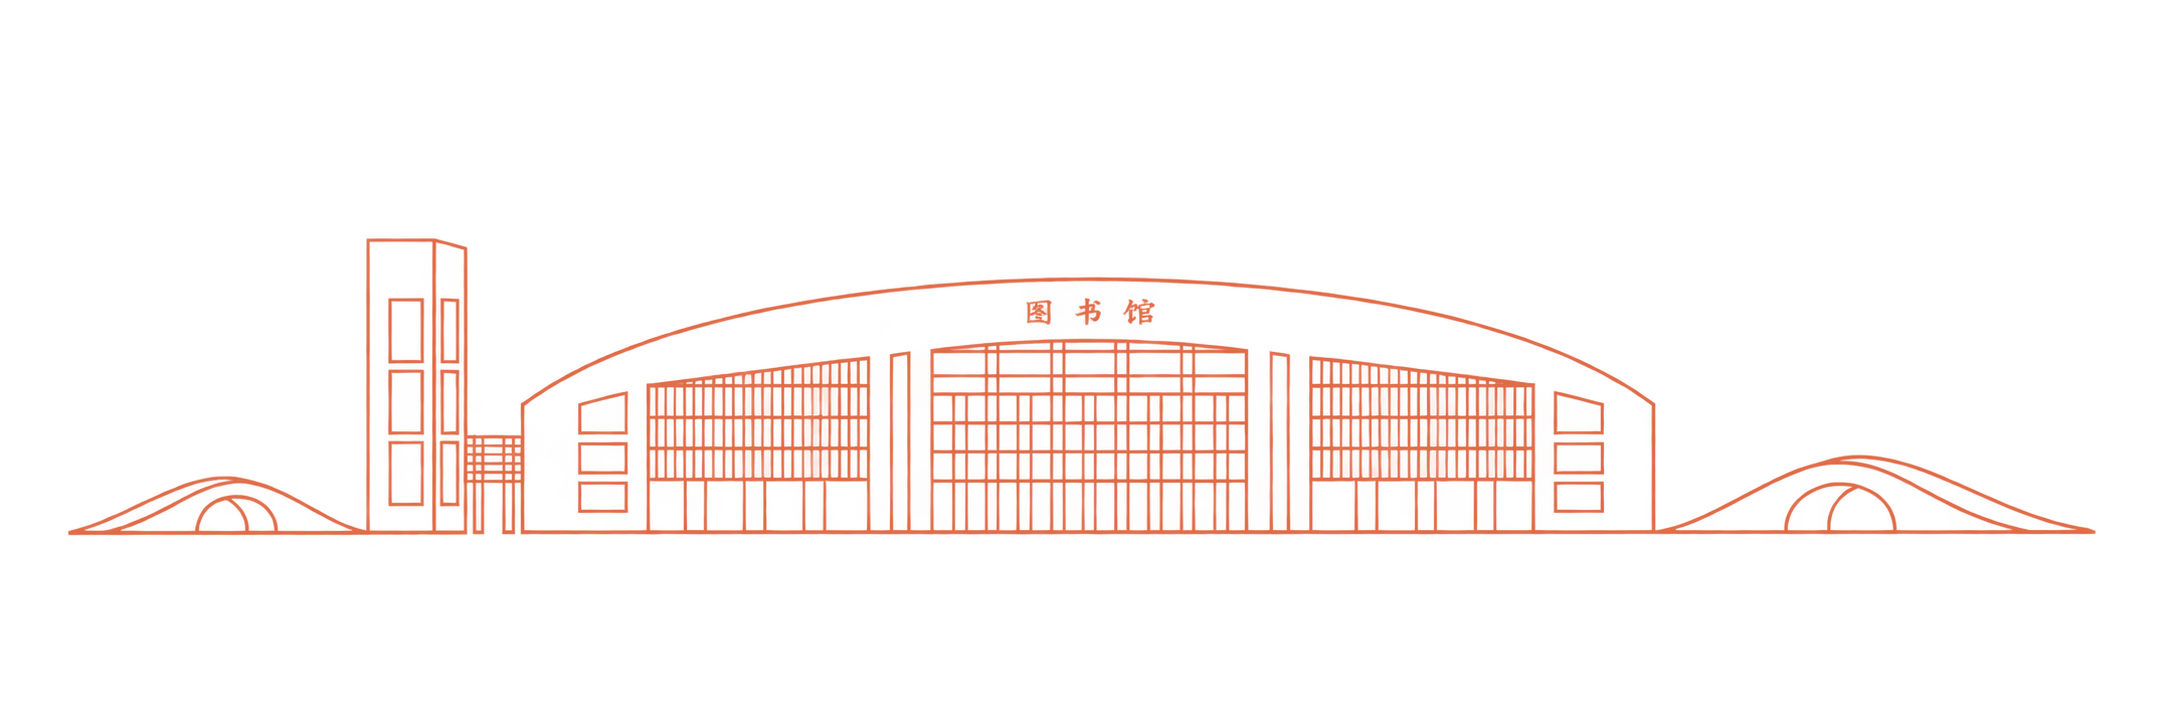
\includegraphics[width=\textwidth]{building-library.png}
        \caption{Line-art campus building}\label{fig:library}
      \end{figure}
    \end{column}
    \begin{column}{0.45\textwidth}
      \small
      \begin{itemize}
        \item Captions are numbered automatically in theme colours;
        \item Figures mix freely with text in columns;
        \item Assets are kept in the \texttt{figures/} folder;
        \item Cross-reference in text: see Fig.~\ref{fig:library}.
      \end{itemize}
    \end{column}
  \end{columns}
\end{frame}

\subsection{Side-by-side Figures}

\begin{frame}{Side-by-side Figures and Cross-references}
  \begin{columns}[T]
    \begin{column}{0.48\textwidth}
      \begin{figure}
        \centering
        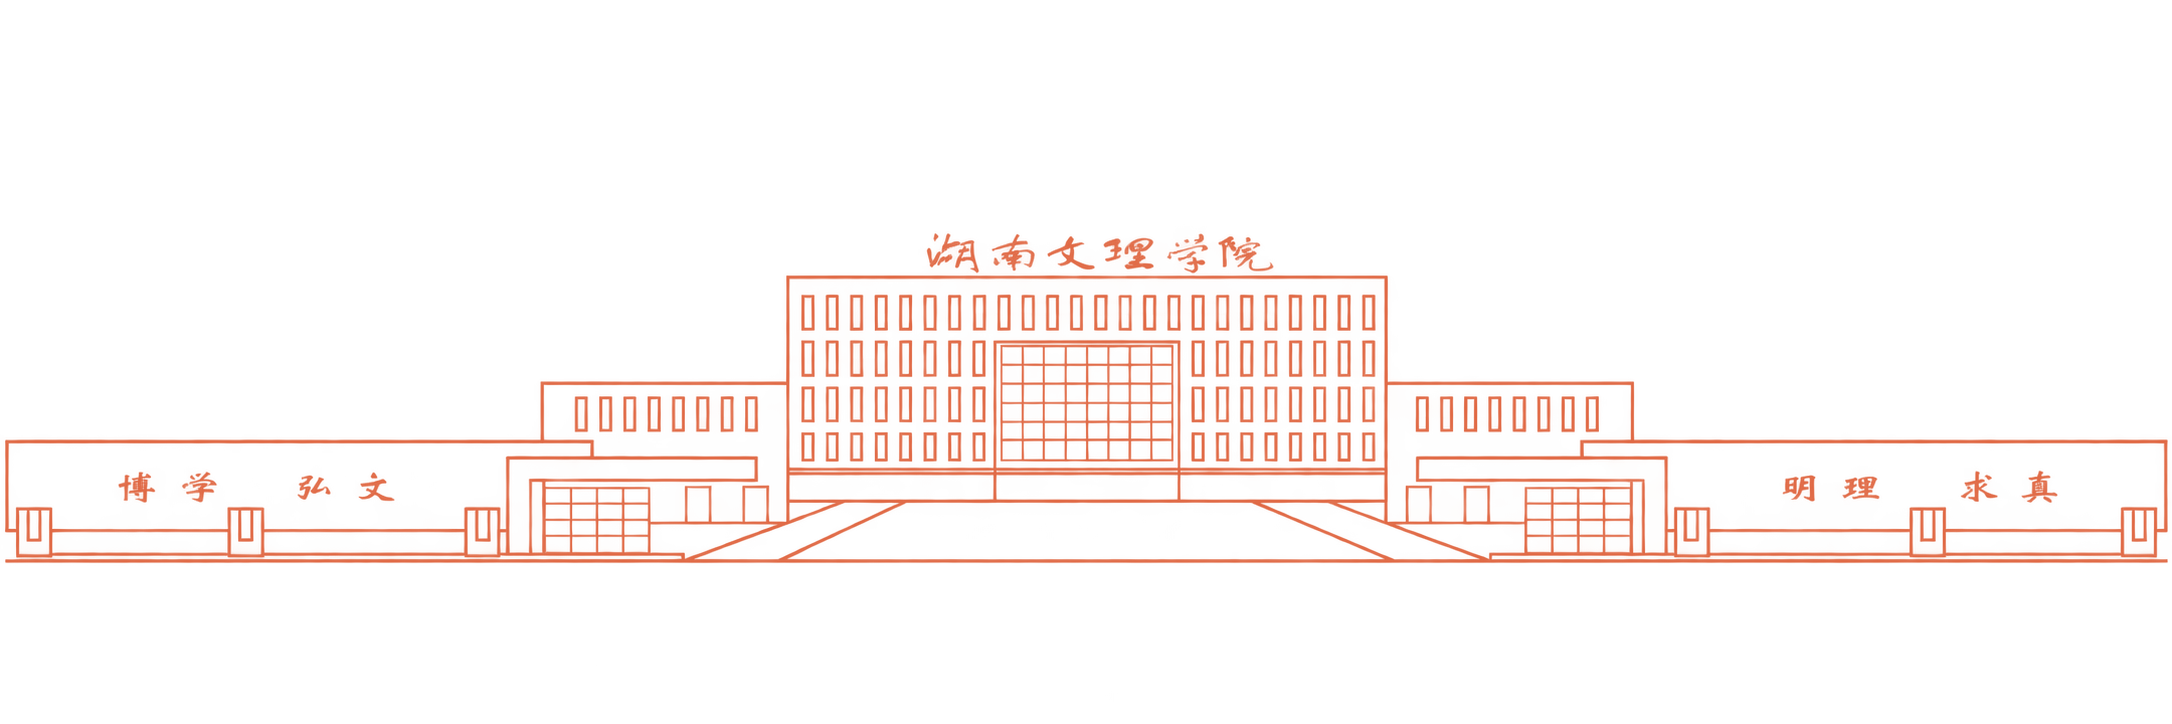
\includegraphics[width=\textwidth]{building-gate.png}
        \caption{Side-by-side figure 1 (line art)}\label{fig:gate}
      \end{figure}
    \end{column}
    \begin{column}{0.48\textwidth}
      \begin{figure}
        \centering
        
\includegraphics[width=0.5\textwidth]{huas-badge.png}
        \caption{Side-by-side figure 2 (badge)}\label{fig:badge}
      \end{figure}
    \end{column}
  \end{columns}
  \vskip1ex
  {\small Fig.~\ref{fig:gate} and Fig.~\ref{fig:badge} sit side by side in one
    row; cross-references update automatically as floats are added or removed,
    \alert{\textbf{with no manual maintenance}}.}
\end{frame}

%% ==================== 3. Blocks, Theorems and Formulas ====================
\section{Blocks, Theorems and Formulas}

\subsection{Block Environments}

\begin{frame}{The Three Block Environments}
  \begin{block}{Work summary (block)}
    Dataset construction, reproduction of three baselines and design of the
    comparative study are completed; an interim report is available.
  \end{block}
  \begin{exampleblock}{Result example (exampleblock)}
    On the public dataset, the proposed method improves accuracy by
    3.2 percentage points over the best baseline.
  \end{exampleblock}
  \begin{alertblock}{Risks and remedies (alertblock)}
    Tight schedule: keep a two-week buffer; if data are insufficient, switch to
    a public benchmark dataset.
  \end{alertblock}
\end{frame}

\subsection{Theorems and Proofs}

\begin{frame}{Theorem, Proof and Example}
  \begin{theorem}[Pythagorean theorem]
    In a right-angled triangle, the sum of the squares of the two legs equals
    the square of the hypotenuse.
  \end{theorem}
  \begin{proof}
    Let the legs be $a,b$ and the hypotenuse $c$. Arrange four congruent copies
    of the triangle into a square of side $a+b$; comparing the two area
    decompositions yields $a^2+b^2=c^2$.
  \end{proof}
  \begin{example}
    For $a=3$ and $b=4$ we get $c=\sqrt{a^2+b^2}=5$.
  \end{example}
\end{frame}

\subsection{Formulas}

\begin{frame}{Inline and Display Equations}
  \small
  Inline math: the objective is $J(\theta)$, the learning rate is
  $\alpha=0.05$, and the sample size is $n=320$.
  \[ k:[-\pi,\pi]\rightarrow[0,1] \]
  Numbered equation: the network input is an image tensor
  \begin{equation}
    \mathbf{x}\in\mathbb{R}^{C_{\text{in}}\times H\times W}
    \label{eq:input}
  \end{equation}
  where $C_{\text{in}}$ is the number of channels, $H$ the height and $W$ the
  width; Eq.~\eqref{eq:input} determines the tensor shapes of each layer.
\end{frame}

\begin{frame}{Multiline Equations and Cases}
  \begin{columns}[T]
    \begin{column}{0.52\textwidth}
      \small Aligned equations (align):
      \begin{align}
        Q_{\text{target}} &= r+\gamma\,Q^{\pi}(s',\pi_\theta(s'))+\epsilon,\\
        \epsilon &\sim \mathrm{clip}\bigl(\mathcal{N}(0,\sigma),-c,c\bigr).
      \end{align}
    \end{column}
    \begin{column}{0.45\textwidth}
      \small Piecewise function (cases):
      \[ L(e)=\begin{cases}
        e^{2}, & |e|\le 1;\\
        2|e|-1, & |e|>1.
      \end{cases} \]
    \end{column}
  \end{columns}
  \vskip1ex
  {\small Here $r$ is the immediate reward, $\gamma$ the discount factor and
    $Q^{\pi}$ the action-value function; $L(e)$ is a robust loss that varies
    piecewise with the error $e$.}
\end{frame}

%% ==================== 4. Tables, Code and Summary ====================
\section{Tables, Code and Summary}

\subsection{Tables and Code}

\begin{frame}{Tables with Coloured Headers}
  \begin{table}
    \centering\small
    \caption{Unique-value counts per field (sample)}\label{tab:unique}
    \begin{tabular}{lc}
      \huastableheader % colored header row (macro provided by huasbeamer)
      \huastableheaderfont Field & \huastableheaderfont \# unique values \\
      \midrule
      \texttt{posting\_id} & 34250 \\
      \texttt{image} & 32412 \\
      \texttt{image\_phash} & 28735 \\
      \texttt{title} & 33117 \\
      \texttt{label\_group} & 11014 \\
      \bottomrule
    \end{tabular}
  \end{table}
  \vskip1ex
  {\small Tab.~\ref{tab:unique} uses \texttt{booktabs} rules together with the
    \texttt{\textbackslash huastableheader} macro; row spacing is set centrally
    by the template, and \texttt{multirow}/\texttt{multicolumn} merge cells.}
\end{frame}

\begin{frame}[fragile]{Code Listings}
  \begin{columns}[T]
    \begin{column}{0.55\textwidth}
\begin{lstlisting}[language=TeX]
\begin{itemize}
  \item Data collection and preprocessing
  \item Model design and training
  \begin{itemize}
    \item Feature extraction and tuning
  \end{itemize}
\end{itemize}
\end{lstlisting}
    \end{column}
    \begin{column}{0.42\textwidth}
      \small
      Rendered result:
      \begin{itemize}
        \item Data collection and preprocessing
        \item Model design and training
        \begin{itemize}
          \item Feature extraction and tuning
        \end{itemize}
      \end{itemize}
      \vskip0.8ex
      {\footnotesize Keywords, comments and strings are coloured separately;
        line numbers appear on the left, and long lines wrap automatically
        (\texttt{breaklines}).}
    \end{column}
  \end{columns}
\end{frame}

\subsection{Citations and Navigation}

\begin{frame}{Citations and Footnotes}
  \begin{block}{Citation examples}
    \begin{itemize}
      \item Single citation: a survey of data-driven methods\cite{zhang2023};
      \item Multiple citations: training methods and typesetting
        tools\cite{chen2022,li2020};
      \item Citations often go with footnotes to trace data sources and
        remarks\cite{wang2021,gao2024}.
    \end{itemize}
  \end{block}
  \begin{exampleblock}{Quotation and footnote}
    \begin{quote}\small
      ``Good tools are a prerequisite to the successful execution of a job.''%
      \footnote{Quotation example: footnotes are placed at the page bottom.}
    \end{quote}
  \end{exampleblock}
  {\small References are managed with \texttt{bib\LaTeX} and numbered
    automatically; full entries appear on the References pages
    (\texttt{allowframebreaks} splits them if needed).}
\end{frame}

\begin{frame}{Hyperlinks and Navigation}
  \begin{columns}[T]
    \begin{column}{0.52\textwidth}
      \small
      \begin{description}
        \item[\texttt{url}] \url{https://www.huas.cn/}
        \item[\texttt{href}] \href{https://www.huas.cn/}{Hunan University of Arts and Science}
        \item[\texttt{jump}] \hyperlink{frame:gallery}{Jump to the element gallery}
      \end{description}
    \end{column}
    \begin{column}{0.45\textwidth}
      \small
      \begin{itemize}
        \item Cross-references: Fig.~\ref{fig:library},
          Tab.~\ref{tab:unique}, Eq.~\eqref{eq:input};
        \item Bottom-right: navigation buttons and page numbers;
        \item TOC entries and bibliography items are clickable.
      \end{itemize}
    \end{column}
  \end{columns}
\end{frame}

\subsection{Summary and Outlook}

\begin{frame}{Element Gallery}
  \hypertarget{frame:gallery}{}
  \begin{table}
    \centering\scriptsize
    \caption{Layout elements covered by this demo}\label{tab:gallery}
    \begin{tabular}{lll}
      \huastableheader
      \huastableheaderfont Category & \huastableheaderfont Environments/commands &
      \huastableheaderfont Example pages \\
      \midrule
      Lists & itemize / enumerate / description & Multilevel and description lists \\
      Layout & columns / figure / caption & Columns, text and figures \\
      Blocks & block / exampleblock / alertblock & The three block environments \\
      Theorems & theorem / proof / example & Theorem and proof \\
      Math & equation / align / cases & Inline, display and multiline \\
      Tables & tabular + huastableheader & Coloured header rules \\
      Code & lstlisting & Code listings \\
      Refs & cite / footnote / hyperlink & Citations and navigation \\
      \bottomrule
    \end{tabular}
  \end{table}
\end{frame}

\begin{frame}{Closing Remarks}
  \begin{block}{What the template gives you}
    \begin{itemize}
      \item Consistent colours, fonts, headers, footers and decorations;
      \item All common layout elements are pre-styled and ready to use.
    \end{itemize}
  \end{block}
  \begin{exampleblock}{Suggestions}
    \begin{itemize}
      \item Write your content first, then apply the layout; any slide here can
        be copied and rewritten;
      \item For fine tuning, search the starred comments in
        \texttt{huasbeamer.sty};
      \item The cool blue-white scheme only needs the \texttt{blue} theme option.
    \end{itemize}
  \end{exampleblock}
\end{frame}

%% ---------------- References ----------------
\begin{frame}[allowframebreaks]{References}
  \footnotesize
  \bibliographystyle{plain}
  \bibliography{reference}
\end{frame}

%% ---------------- Acknowledgements / Q&A ----------------
\begin{frame}[plain,noframenumbering]
  \begin{tikzpicture}[remember picture,overlay]
    \shade[left color=huasdeep,right color=huasorange]
      (current page.south west) rectangle (current page.north east);
    \node[anchor=south,opacity=0.16] at ([yshift=0.35cm]current page.south) {%
      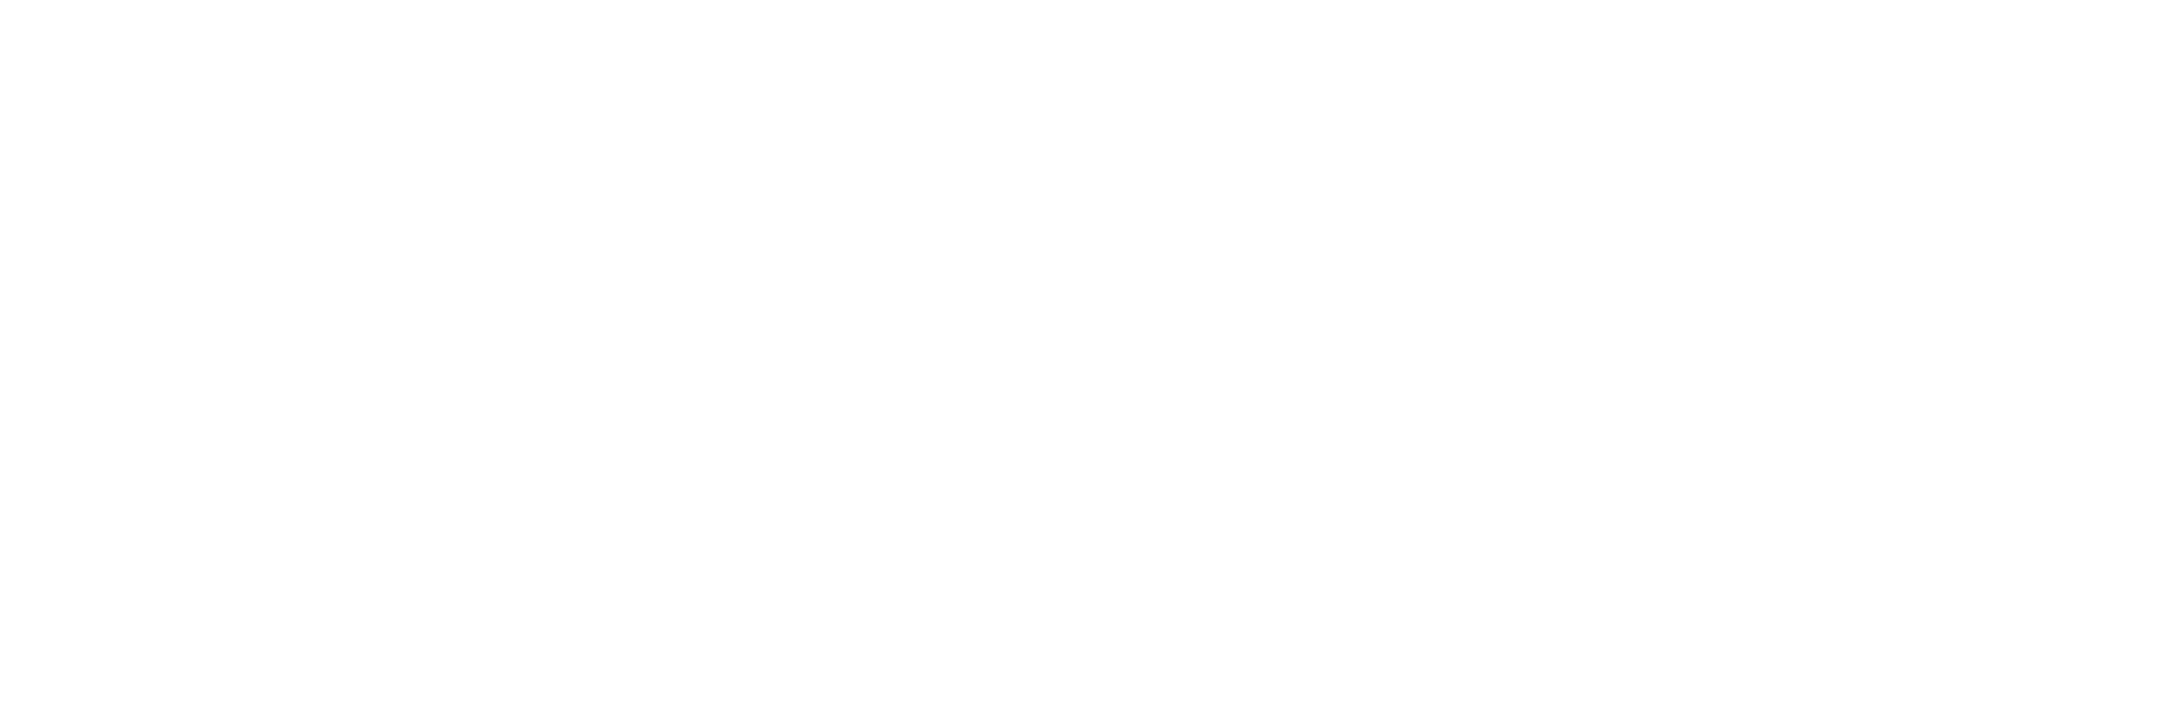
\includegraphics[width=1.04\paperwidth]{building-gate-white.png}};
  \end{tikzpicture}
  \vskip2.2cm
  \begin{center}
    {\Huge\bfseries\color{white}Thank You!}\\[1.8ex]
    {\large\color{white}Q \& A}\\[1.5ex]
    {\footnotesize\color{white!70}Hunan University of Arts and Science}
  \end{center}
\end{frame}

\end{document}
